\documentclass{article}

\usepackage[T1]{fontenc} 
\usepackage{bm} %\bm{} bold math
\usepackage{tikz} % for tikzpictures
\usepackage{amsmath, amssymb}
\usetikzlibrary{positioning, calc} % For better label positioning

\usepackage{caption} %for captionof{figure} in Figure enviorment

\usepackage{multicol} %for multiple columns
\usepackage{float} %for [H] for floats in muticols

% figures in multicols
\newenvironment{Figure}
  {\par\medskip\noindent\minipage{\linewidth}}
  {\endminipage\par\medskip}

\usepackage{geometry}
\geometry{
    left = 1cm,
    right = 1cm, 
    top = 1cm,
    bottom = 2cm
}

\usepackage{biblatex}
\addbibresource{Bibliography.bib}

\usepackage{siunitx}

\usepackage{ mathrsfs } % for mathscr fro L of likelyhood
\newcommand{\Like}{\mathscr{L}}
\newcommand{\Prior}{\mathbb{P}}
\newcommand{\Posterior}{\mathbb{P}}


\title{Rotational Velocity in the Milky Way}
\author{Colombo Gabriele, Maszkowski Michal, Seghezzi Daniele}
\date{\today}

%%%%%%%%%%%%%%%%%%%%%%%%%%%%%%%%%%%%
\begin{document}

%%%%%%%%%%%%%%%%%%%%%%%%%
% frontmatter not in multicols
\maketitle

\section*{Abstract}

%In this excercise we aim to model the rotation of stars within the Milky Way around its center. 
In this report we present a model for the rotation of stars in the Milky Way around its center.
%We introduce an inertial frame of reference centered at the center of the galaxy, with xy-plane coinciding with the galactic plane and x-axis pointing away from the Sun. We will denote it as CG frame.
In a fisrt simpler model, we assume that the stars in the GC (Galactic Center) frame move in circular orbits around its origin with a constant velocity $V_{\text{rot}}$, as well as the LSR (Local Standard of Rest), and that the Sun frame is moving with a velocity $U_{\odot}$ in the x-direction and $V_{\odot}$ in the y-direction in the GC frame with respect to the LSR (figure~\ref{fig:FrameOfReference}). Then, we present a second, more complex model, in which we add, for each star, a random component $v_{\text{rand}, i} \sim N(0, \sigma)$ to its radial velocity, accounting for their random motion.

%We are going to assume that also LSR (Local Standard of Rest) is moving with a velocity $V_{\text{rad}}$ in the y-direction in the CG frame.
%We also introduce a frame of reference centered at the Sun, with the x-axis pointing towards the center of the galaxy, and the z-axis pointing towards the North Galactic Pole. We will denote it as Sun frame.
%The Sun frame is rotating with an angular velocity $w$ around the z-axis due to the rotation of the galaxy with respect to the CG frame.

% In both cases we aim to model the velocity of stars in the radial direction in the Sun frame of reference.
% and find $V_{\text{rad}}$, $U_0$ and $V_0$ using Baysian Inference on the data provided by the GAIA mission.

In this report, we use data provided by GAIA DR2~\cite{GAIADR2}.
For each star on the galactic plane we consider its longitude, parallax, and radial velocity, with respect to the Sun frame of reference.
We also consider the provided uncertainties of the measurements of parallax and radial velocity.

By means of Bayesian inference on the data we find the distributions of parameters of the two models, namely $\mathbf{\theta_1} = (V_{\text{rot}}, U_{\odot}, V_{\odot})$ and $\mathbf{\theta_2} = (V_{\text{rot}}, U_{\odot}, V_{\odot}, \sigma)$.
We used MCMC (Monte Carlo Markov Chain) with emcee package in python~\cite{EMCEE} to estimate the non-normalized posterior of the two models. 

In the first model, we estimate the parameters and their 95\% confidence interval to be: % put this into a table in Data analysis:
$V_{\text{rot}} = 211.45_{-0.04}^{+0.04}$ \unit{\kilo\meter\per\second};  
$U_{\odot} = 11.638_{-0.005}^{+0.005}$ \unit{\kilo\meter\per\second};  
$U_{\odot} = 21.604_{-0.005}^{+0.005}$ \unit{\kilo\meter\per\second}.  
With the second model instead, we got:  
$V_{\text{rot}} = 204_{-2}^{+2}$ \unit{\kilo\meter\per\second};  
$U_{\odot} = 11.7_{-0.3}^{+0.3}$ \unit{\kilo\meter\per\second};  
$U_{\odot} = 21.7_{-0.3}^{+0.3}$ \unit{\kilo\meter\per\second};  
$\sigma = 30.6_{-0.2}^{+0.2}$ \unit{\kilo\meter\per\second}.  



%%%%%%%%%%%%%%%%%%%%%%%%%
% mainmatter in multicols (save some space)
\begin{multicols}{2}
\section{Datas}

In this work we will use data taken from GAIA DR2~\cite{GAIADR2}. From the vast dataset of stars analyzed by GAIA, we first select only those for which radial velocities, $v_{\text{rad}}$, were measured relative to the Sun using the Doppler effect. To manage the dataset size efficiently, we then apply a random selection to significantly reduce the quantity of data, imposing the random index of data to be less than 100000000. 

For each selected star, we extract key parameters from GAIA DR2, including parallax $p$ and its associated error $\sigma_{\text{p}}$, radial velocity $v_{\text{rad}}$ with its measurement uncertainty $\sigma_{\text{v}}$, and galactic coordinates, i.e. latitude $b$ and longitude $l$.

To focus our analysis on stars located within the galactic plane, we impose a selection criterion of $\vert b \vert < 5^{\circ}$. Additionally, to ensure the reliability of the data, we retain only stars with a relative parallax error smaller than 20$\%$ and a radial velocity error below 5 \unit{\kilo\meter\per\second}. % this is a section on its own

\section{Model}
In this section we present the physical and the statistical models we developed for the study of the Galactic kinematics of the Milky Way. Our physical assumptions, presented in the paragraph~\ref{subsec:PhysicalModel}, lead to a prediction for the radial motion of stars with respect to the Sun as a function of their longitude $l$ and parallax $p$. The prediction, for each star, can then be compared to the direct measurement. In the paragraph~\ref{subsec:StatisticalModel} we formally present our statistical assumptions on the data and the parameters of the two models with their priors and likelihoods.

\subsection{Physical Model}

In our model, the Sun's frame moves around the Galactic Center GC with a drift velocity (that of the Local Standard of Rest LSR) plus a random vector. The drift velocity of the LSR in this model is considered in module equal to the drift velocities of each star in our galaxy and analyzed by GAIA DR2
In the following, primate vectors are in the frame of reference of the Sun, whereas unprimed ones are in the frame of reference of the center of the galaxy. Angles are supposed to be expressed as radians. 
Calling $\bm{v}_0$ the total velocity of the Sun relative to the center of the galaxy, we have the following relation:

\begin{equation}\label{eq:SunVelocity}
    \bm{v}_0 = \bm{v}_{LSR} + \bm{v}_{rand}
\end{equation}

\noindent
We can fix the frames of reference in the center of the Galaxy and on the Sun as in fig.\ref{fig:FrameOfReference}. In the picture, all the velocities are represented in the frame of reference fixed at the center of the galaxy. In our model, in this frame, all the stars (and the LSR frame) move around the center with velocity $V_{rot}$, therefore, the velocity for a star s at angle $\varphi$ from the x-axis is:

\begin{equation}\label{eq:VComponents}
    \begin{aligned}
        \bm{v}_s &= V_{rot} (-\hat{e}_{\varphi}) \\
        \hat{e}_{\varphi} &= \begin{pmatrix} -\sin(\varphi) \\ \cos(\varphi) \end{pmatrix}
    \end{aligned}
\end{equation}

\noindent
In particular, we fix $\varphi = \pi$ for the Sun. Therefore, the velocity of the Sun, in the rest frame of the Galaxy is given by the equation:

\begin{equation}\label{eq:VSun}
    \bm{v}_0 = \begin{pmatrix} 0 \\ V_{rot} \end{pmatrix} + \begin{pmatrix} U_0 \\ V_0 \end{pmatrix}
\end{equation}
 
\noindent
The frame of reference of the sun is moving with velocity $\bm{v}_0$ given by eq.\ref{eq:SunVelocity}, and its axis are rotating with an angular velocity $\bm{w}_{sun} = -w_{sun} \hat{e}_z$. Therefore, the velocity $\bm{v'}_s$ of a star s at distance $d$ from the Sun is given by the equation
\begin{equation}\label{eq:ReferenceFrame}
    \bm{v}_s' = \bm{v}_s - \bm{v}_0 - \bm{w}_{sun} \times \hat{e}_r' d = \bm{v}_s - \bm{v}_0 + w_{sun} \hat{e}_l' d
\end{equation}
\noindent 


\noindent 
The radial component of the velocity of a star with longitude l in the sun frame of reference is finally given by:

\begin{equation}\label{eq:VSunRad}
    \begin{aligned}
        \hat{e}_r' &= \begin{pmatrix} \cos(l) \\ \sin(l) \end{pmatrix} \\
        v_s^{\text{rad}'}  &= \bm{v}_s' \cdot \hat{e}_r' = \\ 
        &=V_{rot} \biggl[ \sin\varphi \cos l - (1 + \cos\varphi)\sin l \biggr] - U_0 \cos l - V_0 \sin l
    \end{aligned}
\end{equation}
\noindent
%Note that the rotation of the axis of the frame of reference of the Sun contributes only to the longitudinal component of the relative velocities of stars since $\hat{e}_r' \cdot \hat{e}_l' = 0$.


\input{CCTikzPicture.tex}

Eq.\ref{eq:VSunRad} must be adapted to the actual data provided by GAIA, which means expressing $sin\varphi$ and $cos\varphi$ in terms of $l$ and the parallax $p$, expressed in arcoseconds. First of all, the distance in parsec can be computed as:

\begin{equation}\label{eq:DistanceParallax}
    d[pc] = \frac{1000}{p[arcsec]}
\end{equation}

\noindent
Then, by applying the cosine theorem two times for $R, d, D, l, \varphi$ (fig.\ref{fig:FrameOfReference}), $cos\varphi$ can be written as:

\begin{equation}\label{eq:CosPhi}
    \cos\varphi = \frac{d \cos l - R}{\sqrt{d^2 + R^2 - 2dR \cos l}}
\end{equation}

\noindent
and, therefore,

\begin{equation}\label{eq:SinPhi}
    \sin\varphi = \pm \sqrt{1 - \cos^2 \varphi} = \frac{d\sin l}{\sqrt{d^2 + R^2 -2dR \cos l}}
\end{equation}
\noindent
By substituting eq.\ref{eq:DistanceParallax}-\ref{eq:SinPhi} into eq.\ref{eq:VSunRad}, we get an expression for the prediction of the model for the radial component of the velocity of star $i$ $v_{rad}^{mod}(l_i, p_i)$ as a function of the measurements of its longitude and parallax $l_i, p_i$.

\subsection{Statistical Model}\label{subsec:StatisticalModel}
In the following we describe the Bayesian inference we have made on the parameters of the two models. 
We used Monte Carlo Markov Chains (MCMC) provided by the emcee package in python 
to get an approximation of the non-normalized posteriors of our models 
$\Posterior^{*}(\theta \vert \mathcal{D})$, considering only the numerator of Bayes' theorem (posterior):

\begin{equation}\label{Eq:NonNormPosterior}
    \Posterior^{*}(\theta \vert \mathcal{D}) = \Like(\mathcal{D} \vert \theta) \Prior(\theta)
\end{equation}

\noindent where $\Like(\mathcal{D} \vert \theta)$ is the likelihood and $\Prior(\theta)$ is the prior. In practice, the logarithms of these quantities were used to achieve numerical stability.

%write this here to avoid repetitions
In both models, we assumed each measurement and each parameter to be independent of all the others, since there is no a-priori reason to consider them to be correlated. Under this assumption, the likelihood and the prior factorize in the product of individual terms, so, their logarithms are given by the sum of those individual terms. Then, we assume the value $m$ of each measure to be  the sum of its true value, and a random error $\epsilon$, extracted from a normal distribution centered at 0 with standard deviation $\sigma_m$ given by the statistical uncertainty provided by GAIA database ($\epsilon \sim N(0, \sigma_\text{m})$).

For the first model we have a set of three parameters $\mathbf{\theta_1} = (V_{\text{rot}}, U_{\odot}, V_{\odot})$. 
% and for this model we will assume each measurement of the stars' radial velocity 
% to be a random variable sampled from a gaussian distributrion centered at the true value $v_{\text{rad}}$, 
% with standard deviation given by the error reported by GAIA, 
% $\sigma_{\text{v}}$ ($v_{\text{rad}} \sim N(v_{\text{rad}},\sigma_{\text{v}})$). 
% Moreover, we will also assume the measurements to be mutually indipendent. 
% From this two assumptions follow directly that our likelihood will be a product of gaussians. 
% So the log-likelihood for this model is:
Neglecting the uncertainties associated to the parallax measurements, the difference between the measure of the radial velocity $v_{\text{rad}, i}$ and its prediction $\hat{v}^{(1)}_{\text{rad}, i}$ is a random variable extracted from a normal distribution centered in 0, with standard deviation only given by the statistical uncertainty on the measurements of the radial velocity $\sigma_{\text{v},i}$. 
The log-likelihood of this model therefore is given by the sum of independant terms as:

\begin{equation}\label{Eq:LogLikeMod1}
    \log \Like^{(1)}(\mathcal{D} \vert \theta_1) = -\frac{1}{2}\sum_i[\log(2\pi\sigma_{\text{v},i}^2)+\frac{(v_{\text{rad},i} - \hat{v}_{\text{rad},i}^{(1)})^2}{\sigma_{\text{v},i}^2}]
\end{equation}

%As prior for this model, we firstly assume the three parameters to be indipendent each other, which is pretty realistic since the rotational motion of all the stars shouldn't influence the peculiar motion of the Sun, and its two components on the galactic should be indipendent a priori. For this reason the prior is the product of the priors of each single parameter. 
Then, we chose a flat prior for $V_{\text{rot}}\in[0,\qty{500}{\kilo\meter\per\second}]$, 
in order to include typical values of the rotational motion of stars in spiral barred (Sb) galaxies which are found in the range [144,~330]~\unit{\kilo\meter\per\second}\cite{Schneider2015}. 
For $U_\odot$ and $V_\odot$ we chose a gaussian prior centered in 0, $\log\mathbb{P}^{(1)}(U_\odot) + \log\mathbb{P}^{(1)}(U_\odot) \sim - \frac{U_\odot^2 + V_{\odot}^2}{v_{\text{gal}}^2}$, assuming the peculiar motion of the Sun to be analogous to a stochastic thermal motion. 
%We chose for the standard deviation of these priors to be $v_{\text{gal}}=\qty{200}{\kilo\meter\per\second}$ since, 
% as previously described, these are the order of magnitude for stars speed in galaxies.
As a value for $v_{\text{gal}}$, we chose 200~\unit{\kilo\meter\per\second} since it is the typical scale of stars' velocities in a Sb galaxy.

In our second model, there are four parameters: $\mathbf{\theta_2} = (V_{\text{rad}}, U_{\odot}, V_{\odot}, \sigma)$. 
%As for the measurement of the radial velocities, we also assume the measurement of the stars' parallax to be a random variable sampled from a gaussian distribution centered at the true value $p$, with standard deviation given by the error reported by GAIA, $\sigma_{\text{p}}$ ($p \sim N(p,\sigma_{\text{p}})$). Assuming all the measurements to be independant from one another, the log-likelihood for this model is:
Accounting for the errors on the parallax measurements, the model prediction $\hat{v}^{(2)}_{\text{rad}, i}$ (see equation \ref{eq:VradModel2}) is a random variable extracted from a normal distribution centered in 0 with variance given by the sum of the variance of the random component $\sigma^2$, and the contribution $ {\bigl( \frac{\partial \hat{v}^{(2)}_{\text{rad}, i}}{\partial \text{p}_i} \bigr)}^2 \sigma^2_{\text{p}_i}$ originating from the error on the parallax measurement, 
%Assuming the parallax error to be small, its contribution can be estimated as:
%
% \begin{equation}\label{eq:ParallaxErrorPropagation}
%     \sigma^2_{\text{p}_i -> (2)} = {\biggl( \frac{\partial \hat{v}^{(2)}_{\text{rad}, i}}{\partial \text{p}_i} \biggr)}^2 \sigma^2_{\text{p}_i}
% \end{equation}
%
%\noindent
where the derivative can be computed analytically from equation \ref{eq:VradModel2}.
Then, the difference between the measured value of the radial velocity $v_{\text{rad}, i}$ and the model prediction $\hat{v}^{(2)}_{\text{rad}, i}$ is a random variable extracted from a normal distribution centered in 0 with total variance given by the sum of the variances of the error on the radial velocity measurements, and that on the model prediction, which results in:

\begin{equation}\label{eq:ErrorPropagation}
    \sigma^2_{\text{tot}, i} = \sigma^2_{\text{v},i} +  {\bigl( \frac{\partial \hat{v}^{(2)}_{\text{rad}, i}}{\partial \text{p}_i} \bigr)}^2 \sigma^2_{\text{p}_i} + \sigma^2
\end{equation}

\noindent
As the likelihood factors in independent terms, we get, for its logarithm, the expression:
\begin{equation}\label{Eq:LogLikeMod2}
    \log \mathbb{\Like}^{(2)}(\mathcal{D} \vert \theta_2) = -\frac{1}{2}\sum_i\left\{\log[2\pi(\sigma_{i}^2+\sigma^2)]+\frac{(v_{\text{rad},i} - \hat{v}_{\text{rad},i}^{(2)})^2}{\sigma_{\text{tot}, i}^2}\right\}
\end{equation}

We keep for the first three parameters the same priors decided in the first model, and we assume the fourth parameter $\sigma$ to be uncorrelated to the others. %(stars peculiar motion at a first glance shouldn't depend on the Sun's one either on their average rotational motion). 
The log-prior of the parameter $\sigma$ was chosen as the non-informative prior for the standard deviation of a gaussian~\cite{mackay2003}, since, in our model, it has a similar role:

\begin{equation}\label{eq:LogPriorSigma}
    \log \Prior (\sigma) = - \log(\sigma)
\end{equation}

%GAIA measurements are affected by statistical uncertainties on the evaluations of the parallax and the radial velocity. We assume the measurements to be random variables sampled from a gaussian distributrion centered at the true value of the respective quantity, with standard deviation given by the error reported by GAIA ($v_{rad} \sim N(v_{\text{rad}},\sigma_{\text{v}})$). Assuming the pysical model to be exact, and the measurements to be independant, the difference between the direct measure of the radial velocity, and the corresponding value given by the model by eq.\ref{eq:VSunRad} is a random variable with variance that can be computed through propagation of errors as described in the following. 

\section{DataAnalysis}

\section{Conclusions}

The median values of the posterior probability distributions of the two models, and their 95\% confidence intervals, are reported in table~\ref{tab:parameter_estimates}. It can be observed that the estimates for $U_\odot$ and $V_\odot$ of the two models are compatible with one another, whereas the 95\% confidence interval of the two estimates of $V_{\text{rot}}$ do not overlap. Both estimates of $U_\odot$ are in good agreement with that found in literature~\cite{LocalKinematics}, whereas both estimates of $V_\odot$ are far from being compatible with those in the same ~\cite{LocalKinematics}. The results for $V_{\text{rot}}$ were also compared to those obtained in literature~\cite{GalacticKinematics}. Our estimates result to be lower, but both models yield a non-null overlap of their respective 95\% confidence interval with that of the value found in the literature. The posterior distributions we obtained for the parameters are shown in Appendix~\ref{Appendix:PosteriorDistributions}.
Finally, the middle and lower panels of fig.\ref{fig:DataModelPresentation} present the predictions of the two models, made with the median values obtained for the parameters, using the longitude and parallax of the sample of stars. In the second model, we simulated the contribution of $v_{\text{rand}, i}$ by adding a random number, sampled from a Gaussian centered in 0, with standard deviation given by the median value found for $\sigma$. Visually, it is clear that the second model reproduces the data better than the first one, and that the random motion of stars is crucial to model the radial velocities of stars correctly. 

\begin{table}[H]
    \centering

    \begin{tabular}{l c c | c}
        \hline
        Parameter & Model 1 & Model 2 & Literature\\
        \hline
        $V_{\text{rot}}$ [\unit{\kilo\meter\per\second}] & $211.45_{-0.04}^{+0.04}$ & $204_{-2}^{+2}$ & 225 $\pm$ 10~\cite{GalacticKinematics} \\
        $U_{\odot}$ [\unit{\kilo\meter\per\second}] & $11.638_{-0.005}^{+0.004}$ & $11.7_{-0.3}^{+0.3}$ & $11.1_{-0.8}^{+0.7}$~\cite{LocalKinematics} \\
        $V_{\odot}$ [\unit{\kilo\meter\per\second}] & $21.604_{-0.005}^{+0.005}$ & $21.7_{-0.3}^{+0.3}$ & $12.2^{+0.5}
        _{-0.5}$~\cite{LocalKinematics} \\
        $\sigma$ [\unit{\kilo\meter\per\second}] & --- & $30.6_{-0.2}^{+0.2}$ & --- \\
        \hline
    \end{tabular}
    \caption{Estimated parameters and their 95\% confidence intervals for the two models. The value found in the literature for $V_{\text{rot}}$ is reported with its total uncertainty (one standard deviation), obtained by summing in quadrature the statistical and systematic uncertainties reported in the original article~\cite{GalacticKinematics}.}
    \label{tab:parameter_estimates}
\end{table}



\end{multicols} 

%%%%%%%%%%%%%%%%%%%%%%%%%
% endmatter, not in multicols

\printbibliography
\newpage
\appendix

\section{Posterior distributions}\label{Appendix:PosteriorDistributions}

\begin{figure}[h]
    \centering
    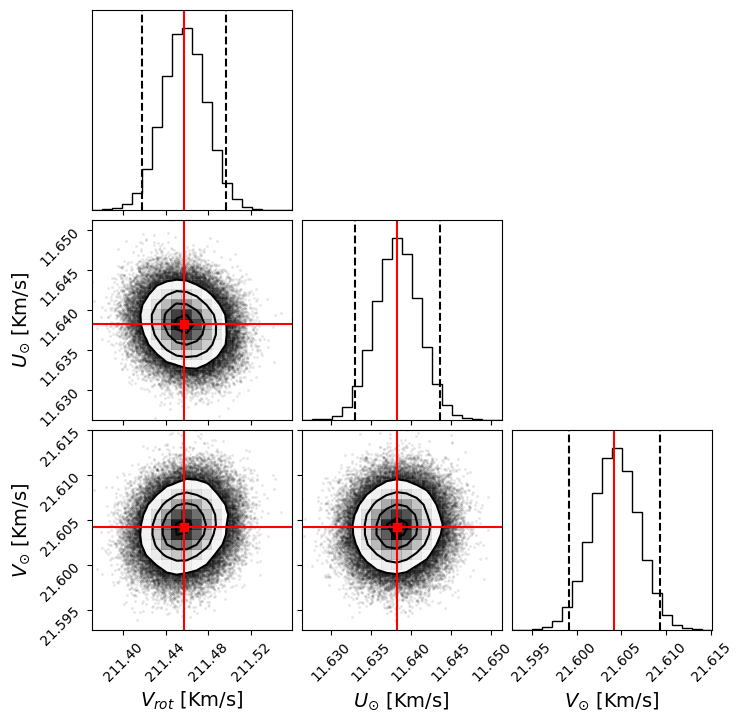
\includegraphics[width = 0.8\linewidth]{Fig/PosteriorSimple.png}
    \caption{Posterior distribution for the parameters of the first model.}\label{fig:PosteriorSimple}
\end{figure}

\begin{figure}[h]
    \centering
    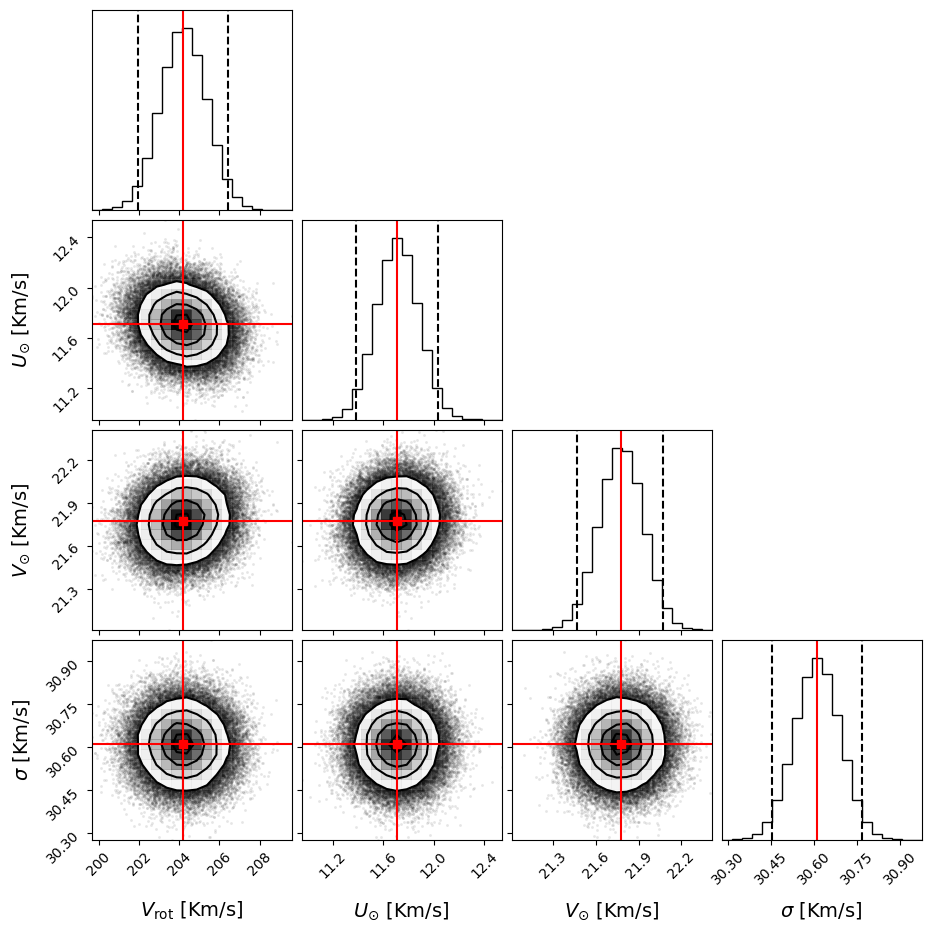
\includegraphics[width = 0.8\linewidth]{Fig/PosteriorFull.png}
    \caption{Posterior distribution for the parameters of the second model.}\label{fig:PosteriorFull}
\end{figure}


\end{document}
